\documentclass[10pt,twocolumn]{article}

\usepackage[letterpaper,margin=0.72in,columnsep=0.25in]{geometry}
\usepackage{amsmath,amssymb}
\usepackage{booktabs}
\usepackage{array}
\usepackage{balance}
\usepackage{graphicx}
\usepackage{microtype}
\usepackage{xcolor}
\usepackage{enumitem}
\usepackage{url}
\usepackage{seqsplit}
\usepackage{xspace}
\usepackage[hidelinks]{hyperref}

\setcounter{dbltopnumber}{2}
\renewcommand{\dbltopfraction}{0.95}
\renewcommand{\dblfloatpagefraction}{0.85}
\renewcommand{\textfraction}{0.05}

\hypersetup{
  pdftitle={AgentLoopGate: Evidence-Governed Evolution and Fail-Closed Selection for Agent Harnesses},
  pdfauthor={JiaoyangLi},
  pdfsubject={Evidence governance for agent harness evolution},
  pdfkeywords={language-model agents, agent harnesses, evaluation governance, reproducibility, DeepSeek Harness}
}

\definecolor{algblue}{HTML}{1D4ED8}
\definecolor{algpurple}{HTML}{6D28D9}
\definecolor{alggreen}{HTML}{15803D}
\definecolor{algred}{HTML}{B91C1C}
\newcommand{\system}{\textsc{AgentLoopGate}\xspace}
\newcommand{\hold}{\textsc{Hold}\xspace}
\newcommand{\ship}{\textsc{Ship-Recommended}\xspace}
\newcommand{\reject}{\textsc{Reject}\xspace}
\newcommand{\code}[1]{\texttt{#1}}
\DeclareRobustCommand{\digest}[1]{\texttt{\seqsplit{#1}}}

\title{\system: Evidence-Governed Evolution and Fail-Closed\\
Selection for Agent Harnesses}
\author{JiaoyangLi\\
\small \href{mailto:jiaoyanglifly@gmail.com}{jiaoyanglifly@gmail.com}\\
\small \url{https://github.com/jiaoyangli-shadow7day/AgentLoopGate}}
\date{Draft -- August 2026}

\begin{document}
\maketitle

\begin{abstract}
Language-model agents can revise prompts, tools, routing, and control flow from
execution failures, but generating a harness change is not evidence that the
change should ship. Aggregate benchmark scores can hide capability exchange;
retries and missing traces can corrupt denominators; and an optimizer may
evaluate its own proposal on coupled data. We present \system, a
runtime-independent evidence and release-governance layer for agent harness
evolution. It preserves the host's native trace, persistence, and telemetry,
then binds content-addressed receipts, normalized runs, immutable snapshots,
cost ledgers, and lineage to frozen objectives, splits, evaluators, pricing,
and gates. External updaters may propose harness candidates, but promotion is
never automatic. The architecture was formed through immutable P0--R14
experiments and incident reviews that successively exposed retry, reply,
lineage, pricing, evaluator, selection, fail-fast, and candidate-validation
defects; these rounds are reported as formation evidence rather than pooled
effectiveness evidence.

In a frozen Banking reference validation with DeepSeek Harness and an external
Agentic Harness Engineering updater, we executed all 125 authorized
pre-release task positions. The baseline and three candidates scored
6/15, 6/15, 5/15, and 6/15 on the identical Selection population. Every
candidate gained task 017 but regressed baseline successes 062 and 095; paired
95\% bootstrap intervals all included zero. \system therefore emitted
\hold, held every candidate, and made zero Release calls. Exact known model
cost was USD~3.908664788, with no unknown model-cost scope. No positive
self-evolution effect is claimed. Headless fixtures further show coexistence
with DeepSeek Harness JSONL/SQLite persistence and OpenTelemetry without
replacing the native session log. The result demonstrates the value of
fail-closed, task-paired governance even when the scientifically correct
outcome is abstention.
\end{abstract}

\section{Introduction}

An agent harness turns a language model into a system that can observe state,
call tools, preserve memory, recover sessions, and interact with users. Recent
work improves such systems through linguistic reflection
\cite{shinn2023reflexion,madaan2023selfrefine}, learned prompt and pipeline
parameters \cite{khattab2023dspy}, function-level optimization
\cite{zhang2024agentoptimizer}, or automated search over agent programs
\cite{hu2024adas}. These methods broaden what can be changed. They do not, by
themselves, establish what evidence is sufficient to release a change.

This distinction matters in stateful, tool-using domains. A candidate may
exchange one capability for another while preserving its aggregate score. A
retry may make a run appear successful while hiding the failed attempt and its
cost. A missing trace or evaluator incident may silently shrink the
denominator. The same data can leak from diagnosis into selection. Finally,
observability data may help debug a system without being complete enough to
serve as release evidence.

We introduce \system, an independent evidence-governance and evolution
decision layer. It is not another runtime, trace backend, or autonomous
deployment system. The host-native execution log remains the source of what
happened. \system adds verifiable references, immutable evaluation identities,
bounded updater inputs, independent baseline-paired selection, and a
lexicographic gate that returns \ship, \hold, or \reject. A human remains the
only promotion authority.

This paper makes four contributions:

\begin{enumerate}[leftmargin=*,nosep]
  \item a runtime-independent evidence model that binds host traces to
  normalized runs, candidates, snapshots, costs, and decisions without
  replacing native persistence or telemetry;
  \item a fail-closed evolution protocol that separates diagnosis,
  Update-Check, baseline-paired Selection, and conditional Release, with exact
  attempt and cost accounting, derived through an auditable P0--R14 sequence
  of failures and versioned controls;
  \item a native DeepSeek Harness plugin that consumes public session events,
  reconciles flush snapshots, preserves JSONL/SQLite and OpenTelemetry, and
  isolates governance failures from the agent turn; and
  \item a fully sealed Banking study showing that two aggregate ties concealed
  two-for-two capability exchanges, for which abstention was the correct system
  outcome.
\end{enumerate}

The empirical claim is deliberately narrow: \system detected unsupported
evolution and stopped it before Release. We do not claim that the external
updater improved the agent, that the result generalizes beyond Banking, or that
fixture latency represents production load.

\section{Problem and Design Goals}

Let $A_0$ be a frozen baseline harness and let an external updater produce
candidates $C_1,\ldots,C_m$ from a bounded failure bundle. For a task $t$ in a
frozen Selection population, $y_t(A)\in\{0,1\}$ denotes stable success under
harness $A$. The release problem is not merely
$\arg\max_A\sum_t y_t(A)$. A candidate should be eligible only when the
evidence population is complete and its gains do not trade away protected
baseline behavior.

\paragraph{Goals.}
The system should (i) accept proposals from multiple updater families without
trusting updater-native scores; (ii) keep diagnosis, selection, and release
data disjoint; (iii) make every conclusion traceable to immutable task, run,
candidate, snapshot, and pricing identities; (iv) treat retries, timeouts,
unknown cost, and infrastructure invalidity as first-class facts; (v) preserve
the host runtime's native operation; and (vi) make abstention a successful
terminal result.

\paragraph{Non-goals.}
\system does not train model weights, certify agent safety, replace host logs,
provide a trace user interface, or deploy a selected candidate. Banking is a
reference validation pack rather than a product boundary.

\paragraph{Trust boundary.}
The trusted kernel contains schemas, canonical serialization, content hashes,
split enforcement, the evaluator interface, candidate registry, attempt and
cost ledgers, and the gate. Updater workspaces and mutable harness assets are
untrusted. Raw model text, user simulation, and external telemetry cannot
declare their own success.

\section{System Design}

\begin{figure*}[t]
\centering
\setlength{\tabcolsep}{3pt}
\renewcommand{\arraystretch}{1.35}
\begin{tabular}{c@{\ $\rightarrow$\ }c@{\ $\rightarrow$\ }c@{\ $\rightarrow$\ }c@{\ $\rightarrow$\ }c}
\fbox{\parbox{0.155\textwidth}{\centering Host-native trace\\Session events / raw result}}
& \fbox{\parbox{0.155\textwidth}{\centering Evidence binding\\Receipt / normalized run}}
& \fbox{\parbox{0.155\textwidth}{\centering Bounded updater\\Candidate / snapshot}}
& \fbox{\parbox{0.155\textwidth}{\centering A0-paired evaluation\\Check / Selection}}
& \fbox{\parbox{0.155\textwidth}{\centering Lexicographic gate\\\ship / \hold / \reject}}
\end{tabular}
\vspace{3pt}

\small Frozen Objective, Split, Evaluator, Pricing, Protocol, and Study identities
bind every transition. Release is created only after Selection returns a
candidate and separate authority is present; promotion is never automatic.
\caption{\system separates runtime facts, governance evidence, candidate
generation, and release decisions. The host trace remains the execution source
of truth; content-addressed governance artifacts refer back to it.}
\label{fig:architecture}
\end{figure*}

\subsection{Evidence planes}

The evidence path has four planes. H0 is the host-native fact source: a
DeepSeek Harness append-only session log or a benchmark raw result. L0 stores a
\emph{SourceTraceRef} and a redacted evidence receipt. L1 stores normalized
run, tool, state, latency, usage, and cost facts. L2 stores evaluation
artifacts: failure bundles, candidate and snapshot manifests, batch summaries,
statistics, lineage, and decisions. Each object uses canonical JSON or YAML and
a SHA-256 digest. Formal conclusions must traverse the chain back to H0.

Telemetry is intentionally not elevated to evaluation truth. OpenTelemetry is
a vendor-neutral framework for traces, metrics, and logs
\cite{opentelemetry2026}; an exporter can be useful yet absent, sampled, or
reconfigured. \system therefore coexists with OTel but bases integrity on the
host session event stream and authenticated receipts.

\subsection{Frozen identities and immutable lifecycle}

A formal experiment freezes the Objective, six isolated task pools, evaluator,
pricing, runtime pins, protocol, study plan, source revision, and baseline
snapshot. Every paid operation first writes a durable \code{STARTED} event and
then exactly one terminal event. Resume verifies existing bytes and continues
only absent work; it cannot silently re-run a paid completed position.

Cost has two distinct questions: whether valid-run comparison cost is exact,
and whether the whole observed attempt surface is complete. Missing cost is
\code{partial} or \code{unavailable}, never zero. Infrastructure-invalid runs
are reported outside the performance denominator and block a batch whose
registered coverage is incomplete.

\subsection{Bounded external updater}

The updater receives only a failure bundle derived from Update-Source plus a
whitelist of mutable parent-snapshot assets. It cannot read Selection or
Release tasks, gold answers, evaluator code, prior private decisions, or the
trusted kernel. Outputs are validated for path scope, schema, semantic
distinctness, runtime capability binding, and lineage before registration.
Updater-native order is retained as evidence but is not a release decision.

\subsection{Baseline-paired selection and conditional release}

Update-Check cheaply rejects malformed or clearly harmful candidates. The
survivors and $A_0$ then run on the identical Selection tasks. For candidate
$C$, define the paired difference $d_t=y_t(C)-y_t(A_0)$, the gain set
$G_C=\{t:d_t=1\}$, and regression set $R_C=\{t:d_t=-1\}$. The R15 correctness
gate required

\begin{equation}
\sum_t d_t > 0, \qquad R_C=\varnothing,
\label{eq:correctness}
\end{equation}

plus complete evidence, zero critical violations, no retry or timeout
increase, p95 latency ratio at most 1.2, and whole-attempt cost ratio at most
1.2. A scalar-score tie is not a gain.

If no candidate satisfies every prerequisite, Selection emits \hold and
forbids Release calls. If a candidate is selected, Release-ID, Release-OOD, and
Replay still require a separately bound execution authorization. Even a final
\ship is a recommendation rather than deployment.

\section{DeepSeek Harness Integration}

DeepSeek Harness is a plugin-composed agent runtime whose durable session log
records the model context, tool calls, and lifecycle events
\cite{deepseekharness2026}. \system integrates as an out-of-tree Cordis bundle
against a pinned developer-preview revision. The Python core remains usable
without the plugin.

The observer subscribes to public session lifecycle and event interfaces. A
live path provides low-latency receipts; each flush reconciles against the
authoritative \code{session.events} snapshot to recover construction, resume,
or transient-buffer gaps. Sequence holes mark evidence incomplete. The plugin
does not register a competing telemetry backend, query private SQLite tables,
or rewrite native JSONL/SQLite. A bridge failure is isolated from the agent
turn but blocks affected evidence from formal decisions. Unload removes tools,
listeners, and the bridge child process.

This arrangement makes native trace and governance evidence complementary.
Developers retain their session persistence and OTel exporter; \system adds
content-addressed provenance and decision semantics.

\section{System Formation and Failure Experience: P0--R14}

\system was not designed in one pass. Its current contracts emerged through a
sequence of frozen experiments, failed preflights, partial batches, and
incident reviews. The repository's experiment identities progress from
\code{EXP\_BANKING\_P0} directly to \code{EXP\_BANKING\_R2}; no registered
\code{EXP\_BANKING\_R1} identity exists. We preserve that naming gap instead of
inventing a run. P0--R14 also cannot be pooled into an effectiveness curve:
protocols, evidence schemas, baselines, and sometimes evaluator inputs changed
between identities. Their legitimate role is process evidence---what failed,
whether the system stopped, what evidence survived, and which control became
mandatory in the successor.

\begin{table*}[!t]
\centering
\footnotesize
\setlength{\tabcolsep}{3.5pt}
\renewcommand{\arraystretch}{1.17}
\begin{tabular}{
  >{\raggedright\arraybackslash}p{0.075\textwidth}
  >{\raggedright\arraybackslash}p{0.205\textwidth}
  >{\raggedright\arraybackslash}p{0.285\textwidth}
  >{\raggedright\arraybackslash}p{0.355\textwidth}
}
\toprule
Round & Terminal evidence & Failure exposed & Control carried forward \\
\midrule
P0--R2 & P0 preserved as superseded \hold; R2 A4 retained a failed protocol
diagnosis & Frozen one-retry intent differed from the invoked runtime default;
stale acceptance, source packaging, ignore rules, and Linux async behavior also
failed clean-room checks & Content-address the execution protocol; supersede
rather than rewrite; require source-artifact and clean-checkout Linux
verification before paid evidence \\
R3 & 22/25 valid Update-Source positions; \hold & Outer resume reapplied the
per-process retry budget, and discarded attempts lost User Simulator cost &
Global per-position attempt cap; append-only task-attempt and independent
Agent/User usage ledgers; unknown cost is never zero \\
R4 & 24/25 valid; \hold; exact whole-attempt model cost USD~0.6917880208 & A
recurrent, uniquely mappable reply wrapper remained unrecognized & Narrow
allow-list normalization only when tool identity and arguments are explicit;
ambiguous syntax still fails closed \\
R5--R6 & R5: 23/25 valid; R6: 24/25 valid; both \hold. R6 reconciled exact
whole-attempt cost USD~0.7698343648 & Reasoning-only empty finals, equal inner
and outer timeouts, additional explicit reply shapes, and indirect failed-call
lineage & One separately ledgered same-session final-only repair; ordered
timeouts; direct task/attempt/session joins; no inference from hidden reasoning \\
R7--R8 & R7 completed Source, created three candidates, and completed A0 Check;
the first candidate Check failed partial. R8 made zero paid calls & Dynamic
pricing produced false exact-zero User cost for nonzero tokens; later audit
found that summaries and gates still read raw rather than direct-ledger cost &
Frozen-price recomputation with a positive-token invariant; direct cost must
propagate through summaries, curves, and final gates end to end \\
R9 & 25/25 Source valid; immutable \hold; exact whole-attempt cost
USD~0.7015112488 & Task 053's golden fixture omitted a required user action,
making a correct trajectory look wrong & Deterministic no-model cause isolation;
versioned evaluator overlay; block candidate generation under contaminated
evidence \\
R10 & 95 formal positions; paid \hold; exact model cost through C2
USD~3.0651904832 & Selection omitted $A_0$, forced a winner, ignored several
whole-attempt operational facts, admitted duplicate candidates, and allowed an
unbound tool route & Same-pool baseline pairing; first-class abstention;
whole-attempt retry/timeout/p95/cost inputs; semantic deduplication and runtime
capability binding \\
R11--R12 & R11: 24/25 Source valid. R12: 34/35 executed positions valid; both
\hold. R12 observed Provider-cost lower bound USD~1.1970712488 & Failed-attempt
sealing lacked direct lineage; a User Simulator empty message and updater use
of process-global \code{/tmp} broke successor execution & Verify-only recovery
for existing bytes; bounded final-only User repair; attempt-local updater
runtime and sandbox doctor; every repair requires a new identity \\
R13 & 24/25 Source valid; \hold. After permanent invalidity, 12 queued positions
still made 588 calls costing a known USD~0.4686327800 & Cross-stage gating
worked, but the serial batch lacked position-level fail-fast & Stop before the
next position after retry exhaustion while retaining the failed position,
unknown cost scope, native trace, and incomplete denominator \\
R14 & 46/125 positions executed; \hold; exact cost USD~1.4876297096. Fail-fast
prevented 79 authorized positions from starting & Candidate precheck inspected
baseline bytes and patch tokens rather than validating materialized prospective
bytes; the only complete candidate Check regressed a baseline success & Apply
each patch in an isolated tree and validate final bytes before registration;
seal a first-class partial \hold; resume is verification-only \\
\bottomrule
\end{tabular}
\caption{System formation through P0--R14. Counts and costs are observed
historical evidence, not comparable estimates of candidate effectiveness.
Every successor retained the predecessor's raw evidence and used a new frozen
identity when execution semantics changed.}
\label{tab:formation-history}
\end{table*}

\paragraph{Execution integrity before optimization.}
P0--R6 showed that an optimizer is premature when a retry can escape its
budget, a discarded call can disappear from cost, or a reply representation can
turn explicit intent into Infrastructure Invalid. The sequence therefore made
attempt topology, timeout ownership, reply normalization, and direct lineage
part of the trusted kernel. Importantly, restoring a parseable or complete
turn did not rewrite business outcomes: repaired positions could remain valid
task failures.

\paragraph{Decision integrity before release.}
R7--R10 moved the fault boundary downstream. Complete execution was still not
enough when dynamic price lookup could create false exact zeros, a summary
could read the wrong cost plane, a broken gold fixture could contaminate the
failure bundle, or Selection could force a winner without a paired baseline.
These incidents produced the frozen-price authority, evaluator versioning,
candidate semantic and capability checks, baseline-paired Selection, and
first-class \hold semantics used in R15.

\paragraph{Fail-fast behavior without evidence deletion.}
R11--R14 tested recovery and stopping behavior. The system repeatedly preserved
partial evidence and refused to fill a missing denominator. R13 quantified a
real efficiency failure inside a serial batch; R14 then demonstrated that the
new position-level stop blocked the remaining queue, while exposing the next
control-plane defect before Selection. This is the practical meaning of
fail-closed evolution: failure is retained as evidence, not hidden to keep the
experiment moving.

Taken together, P0--R14 support a systems claim, not a positive evolution
claim. They show that the architecture was shaped by observable failures and
that each discovered failure was converted into an executable successor
control. R15 is the first complete confirmatory application of the resulting
baseline-bound pre-release policy.

\section{Banking R15 Methodology}

\subsection{Reference environment}

The study uses a knowledge-intensive Banking environment derived from the
$\tau$ family of tool-agent-user benchmarks. Such benchmarks evaluate stateful
conversations, policy following, API use, and final environment state rather
than static text alone \cite{yao2024taubench}. Stateful tool-use evaluation is
also emphasized by ToolSandbox \cite{lu2024toolsandbox}. We use Banking to
exercise the complete evidence path, not to define the domain of \system.

The execution model and user simulator were DeepSeek endpoints under frozen
runtime arguments. The external updater was
\code{agentic-harness-engineering} 0.1.0 at commit
\code{8b2a55d97590363fe50c3cc6b5e833b020a4bb4c}. The benchmark runtime,
protocol, study, source tree, pricing, and $A_0$ were content-addressed before
formal execution.

\subsection{Registered pre-release surface}

R15 executed 25 Update-Source positions, 40 Update-Check positions
($A_0$ plus three candidates, 10 each), and 60 Selection positions
($A_0$ plus three candidates, 15 each): 125/125 authorized positions across
nine complete batches. All positions were valid and no Infrastructure Invalid
run occurred. The experiment contained no Release authorization.

The external updater emitted three semantically distinct candidates in native
order, labeled C1--C3. Selection used stable task success as its primary
endpoint. Latency, critical violations, retries, timeouts, and whole-attempt
cost were gate inputs rather than post hoc diagnostics.

\subsection{Uncertainty and multiplicity}

For each candidate, we bootstrap the 15 paired task differences $d_t$ with
10,000 deterministic resamples and report the nearest-rank 95\% interval for
$\bar d$. The bootstrap seed was preregistered and each comparison derives an
effective content-bound seed. The task, not the trial or model call, is the
statistical unit \cite{efron1979bootstrap}. Intervals are descriptive for the
frozen Selection population: three proposals from one updater are dependent,
and we make neither a multiplicity-adjusted superiority claim nor a
cross-domain inference.

\subsection{Research questions}

We ask whether independent governance (RQ1) detects task-level capability
exchange missed by aggregate scores; whether the system abstains before
Release when no candidate clears the frozen gate (RQ2); whether evidence and
cost remain complete through retries and failures (RQ3); and whether the
DeepSeek Harness plugin coexists with native persistence and OTel in headless
fixtures (RQ4).

\section{Results}

\subsection{Aggregate ties concealed common regressions}

\begin{table*}[t]
\centering
\small
\setlength{\tabcolsep}{5pt}
\begin{tabular}{lrrrrrrl}
\toprule
Variant & Stable & Gains & Regress. & Paired $\bar d$ [95\% CI] & p95 ratio & Cost ratio & Disposition \\
\midrule
$A_0$ & 6/15 & -- & -- & -- & 1.000 & 1.000 & baseline \\
C1 & 6/15 & 017, 096 & 062, 095 & 0.000 [$-$.267, .267] & 1.882 & 1.121 & held \\
C2 & 5/15 & 017, 090 & 056, 062, 095 & $-$.067 [$-$.333, .200] & 1.670 & 1.108 & held \\
C3 & 6/15 & 017, 090 & 062, 095 & 0.000 [$-$.267, .267] & 1.652 & 1.127 & held \\
\bottomrule
\end{tabular}
\caption{Frozen Selection results on the identical 15-task population. Cost
ratio uses whole observed attempt cost; p95 ratio is relative to $A_0$. Every
candidate violated strict gain, zero regression, and p95 non-inferiority.}
\label{tab:selection}
\end{table*}

C1 and C3 tied $A_0$ at 6/15, while C2 scored 5/15. The ties were not stable
equivalence. Every candidate gained task 017 and lost the same baseline
successes 062 and 095; C2 also lost 056. C1 gained an additional task 096,
whereas C2 and C3 gained 090. Thus two aggregate ties represented two gains
exchanged for two protected successes. All paired intervals included zero.

Operational evidence independently disqualified every candidate. All p95
latencies exceeded the 1.2 ratio; C1 added one timeout. Whole-attempt cost
ratios remained within 1.2 but were higher than $A_0$. Because Equation
\ref{eq:correctness} is a prerequisite rather than a weighted score, lower cost
could not compensate for regression.

\begin{figure*}[t]
\centering
\begin{minipage}[t]{0.49\textwidth}
\centering
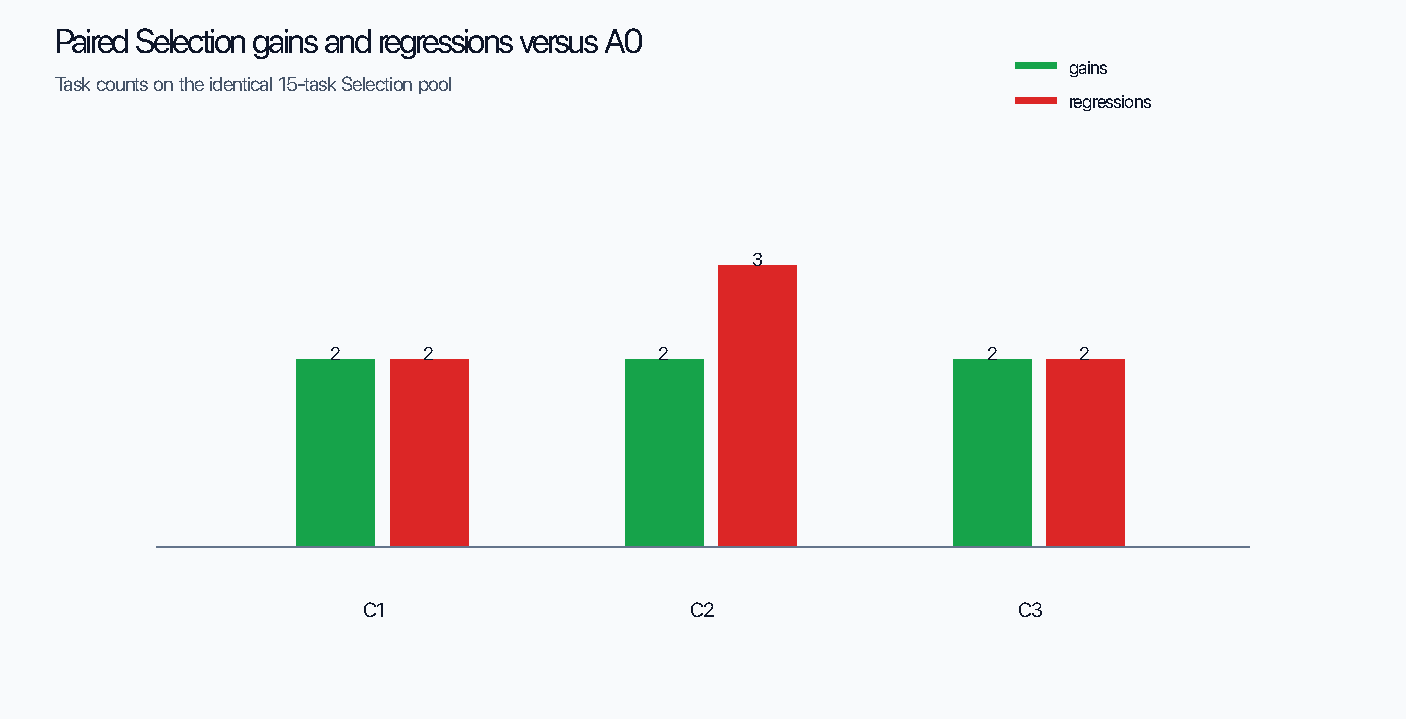
\includegraphics[width=\linewidth]{figures/paired-comparison.pdf}
\end{minipage}\hfill
\begin{minipage}[t]{0.49\textwidth}
\centering
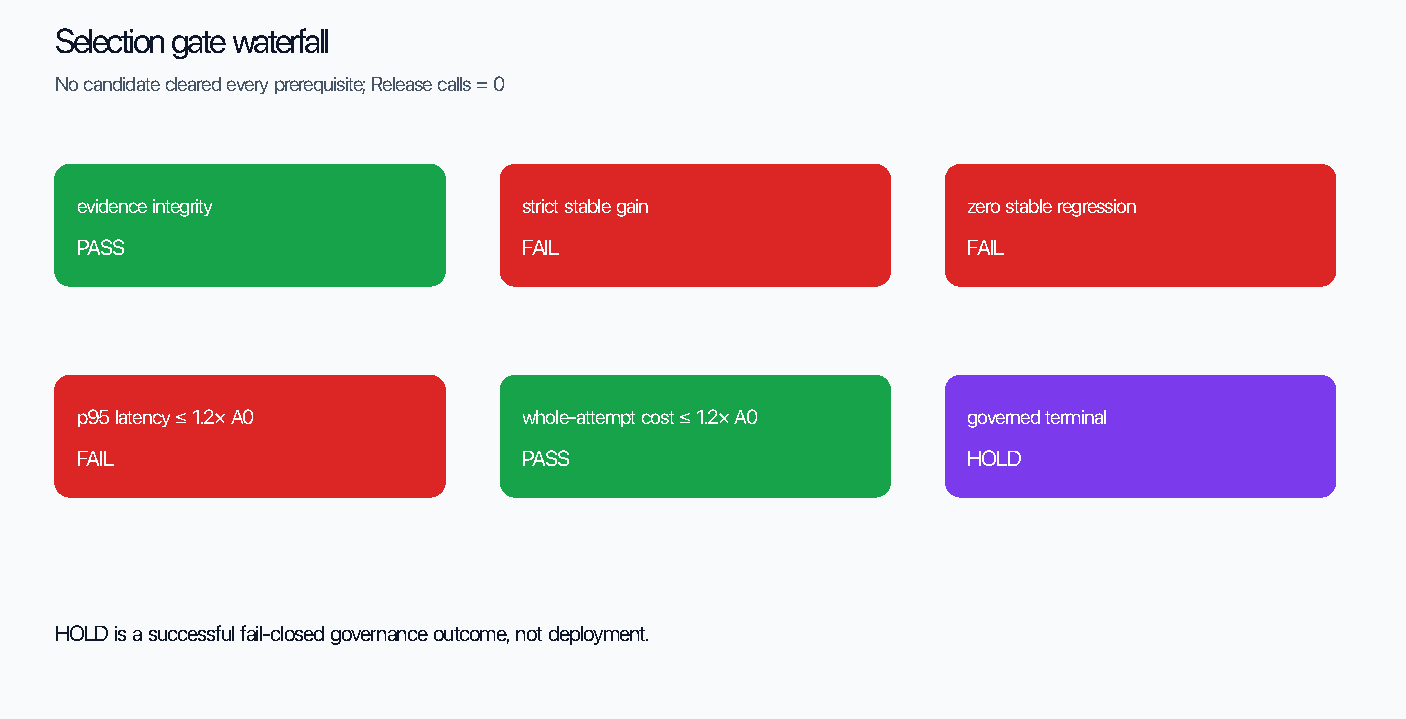
\includegraphics[width=\linewidth]{figures/gate-waterfall.pdf}
\end{minipage}
\caption{Left: candidate gains and regressions relative to $A_0$ on the paired
Selection population. Right: the fail-closed gate outcome. These are
Selection-only figures; Release was not run. Both panels are deterministic
views bound to Selection digest \digest{b5e800...00466}.}
\label{fig:selection}
\end{figure*}

\subsection{The system correctly abstained}

The final reason was
\nolinkurl{no_candidate_passed_baseline_bound_selection_policy}.
\system held C1--C3, set the governed candidate to null, emitted \hold, and
made zero model calls after Selection. No Release-ID, Release-OOD, Replay,
promotion, or deployment artifact exists. This is a normal, successful
terminal state: the system refused to manufacture a winner from a candidate
ladder with unsupported evidence.

RQ1 and RQ2 are therefore answered positively for governance behavior, not for
candidate quality. Independent paired selection changed an updater-native
ranking into abstention, and the conditional Release boundary prevented
additional paid evaluation after a failed prerequisite.

\subsection{Evidence and cost reconciled exactly}

All nine batches carried exact accounting. The call ledger contains 4,378
terminal model calls, 10,343,844 input tokens, 4,648,289 output tokens,
222,019,328 cache-read tokens, zero unresolved calls, and zero provider-level
retries. Task-level retry and timeout facts were separately retained in batch
evidence. Formal batches cost USD~3.8830976464; external updater calls cost
USD~0.0255671416; exact known model cost was USD~3.9086647880. Unknown
model-cost scope was empty. Local compute and GitHub Actions monetary cost were
explicitly unmetered or unavailable, not reported as zero.

The formal process wall time was 52,591.59 seconds (14.61 hours). This duration
includes the deliberately serial, low-concurrency execution path and should
not be read as a minimal achievable runtime. It demonstrates that path,
duration, retries, calls, tokens, and cost can be retained as evidence rather
than reconstructed after the fact.

\subsection{Plugin coexistence passed at fixture scope}

A registered no-model ablation ran 30 paired iterations for each of JSONL and
SQLite persistence with 100 logical session events per iteration. In every
iteration, native persistence survived, the logical session-event hash was
equivalent, observer coverage was complete, and OTel coexistence remained
true. JSONL overhead had p50 $-0.308$~ms and p95 16.424~ms; SQLite overhead had
p50 0.244~ms and p95 0.542~ms. Negative samples reflect local timing noise.
These measurements validate lifecycle coexistence in a headless fixture, not
production throughput or tail-latency service objectives.

A separate synthetic integrity control illustrates gate value: with evaluation
integrity disabled, the fixture would return \ship; the production gate returns
\hold on \code{evaluation\_integrity}. Because this is a synthetic control, it
is evidence of software behavior rather than a causal estimate from R15.

\section{Discussion}

\paragraph{What evolved?}
The external updater produced three real, executable harness proposals, and all
three changed the task-success surface. That is evidence of candidate
generation, not positive evolution. R15 instead identifies a directional
hypothesis: future updaters should treat the stable baseline-success set as
protected constraints and propose sparse, failure-cluster-specific changes.
Testing that hypothesis requires a new frozen identity and untouched
confirmation tasks; R15 cannot validate a mechanism designed after seeing its
Selection failures.

\paragraph{Why not optimize a weighted score?}
A weighted objective permits cost or latency to compensate for correctness
regression. In high-stakes action domains, this can make policy-important
capabilities disappear behind an unchanged average. Lexicographic prerequisites
express the stronger release contract: evidence first, then protected
correctness, then operational non-inferiority. Different applications can
freeze different gates, but changing them after results would require a new
study.

\paragraph{Trace versus telemetry.}
Observability and evaluation evidence overlap but are not identical. Native
session logs answer what the runtime recorded. OTel answers what configured
instrumentation exported. \system keeps the native log authoritative and adds
receipts that are purpose-built for decision completeness. This avoids forcing
developers to abandon existing persistence or exporters.

\paragraph{Negative results as systems evidence.}
Agent-evolution research naturally favors examples where a method improves an
aggregate metric. A governance system should also be evaluated when no proposal
deserves release. R15 exercises the more adversarial branch: plausible,
executable candidates change behavior but fail protected constraints. Correct
abstention, exact accounting, and proof that no Release tail started form the
primary result.

\section{Related Work}

\paragraph{Language-agent improvement.}
ReAct interleaves reasoning and acting \cite{yao2023react}; Reflexion stores
linguistic feedback across trials \cite{shinn2023reflexion}; and Self-Refine
iteratively critiques outputs \cite{madaan2023selfrefine}. DSPy compiles
declarative LM pipelines against metrics \cite{khattab2023dspy}.
AgentOptimizer treats functions as learnable agent parameters
\cite{zhang2024agentoptimizer}, while Automated Design of Agentic Systems
searches over agent programs \cite{hu2024adas}. \system is complementary: it
does not propose a superior optimization algorithm, but constrains inputs,
authenticates outcomes, independently selects proposals, and governs whether
evaluation may advance.

\paragraph{Agent evaluation and tool safety.}
AgentBench evaluates agents across interactive environments
\cite{liu2023agentbench}; $\tau$-bench focuses on tool-agent-user interaction
and reliability \cite{yao2024taubench}; ToolSandbox adds stateful on-policy
tool execution \cite{lu2024toolsandbox}; and ToolEmu uses an emulated sandbox
to identify risky tool behavior \cite{ruan2023toolemu}. \system uses such
benchmark adapters as evidence producers but adds lifecycle, split, lineage,
cost, and release semantics across experiments.

\paragraph{Reproducibility and governance.}
Classical bootstrap methods quantify uncertainty from empirical populations
\cite{efron1979bootstrap}. \system binds the exact population, seed, batch
digests, and comparison artifact so an interval cannot drift independently of
the underlying runs. Its contribution is operational: statistical output is
one prerequisite within a content-addressed decision path, not a substitute
for evidence integrity.

\section{Limitations and Ethics}

R15 covers one Banking environment, one updater backend, one model/runtime
family, three dependent candidates, and a 15-task Selection population.
Bootstrap intervals are correspondingly wide and descriptive. No candidate
reached Release, so there is no Release-ID, OOD, Replay, or cross-domain
effectiveness evidence. The plugin overhead study is a local synthetic fixture
on arm64 macOS, not a production load test. User simulation and provider
variance may affect outcomes. A formal human-factors study of gate review is
also absent.

The study does not expose raw customer or session content. Public artifacts are
sanitized aggregates; raw traces, prompts, model responses, credentials, and
hidden benchmark content remain private. Secret and direct-PII scans are part
of clean-room verification. The system never auto-promotes. These controls
reduce accidental release risk but do not prove safety against a malicious
host, compromised evaluator, or all forms of prompt injection.

\section{Reproducibility and Artifact Availability}

The source tree contains the Python governance core, DeepSeek Harness bundle,
no-key demo, frozen configuration identities, unit and integration tests, and a
sanitized 18-file R15 v1.1 result package. The package independently verifies
without raw traces. Its Manifest digest is
\digest{sha256:79e9a8dd31009f969cdd79021bbcc857c827dc1d5a6808a28fd05937e4f364c8};
the private Outcome digest it binds is
\digest{sha256:827ed2a5b3337832c49cd255f17568fad3a58fe201860311d66decb83ba0bdc3}.

The unified clean-room command runs Python tests and demo, builds an sdist and
wheel, type-checks and tests the plugin, executes headless conformance, packs
the bundle, verifies both R15 packages, and scans the intended public tree for
secrets and direct PII. The repository is prepared at the URL in the title
block; visibility and arXiv submission remain separate owner-authorized
actions at the time of this draft.

\section{Conclusion}

\system separates the ability to generate an agent-harness change from the
authority to release it. Its evidence contracts preserve host-native traces,
its immutable lifecycle makes retries and cost auditable, and its A0-paired
gate makes capability exchange visible. In Banking R15, every updater proposal
gained behavior, every proposal also regressed protected successes, and no
proposal demonstrated a strict stable improvement. The system's correct result
was therefore \hold with zero Release calls. This negative candidate result is
a positive governance result: self-evolution becomes a claim that must be
earned by evidence rather than inferred from an optimizer's output.

\balance
\bibliographystyle{plain}
\bibliography{references}

\clearpage
\onecolumn
\appendix
\section{Evidence Binding}

Table~\ref{tab:bindings} lists the principal content identities used by this
paper. Full values are included so that the manuscript can be checked against
the sanitized package without private execution data.

\begin{table}[h]
\centering
\small
\begin{tabular}{ll}
\toprule
Artifact & Digest or identity \\
\midrule
Experiment & \code{EXP\_BANKING\_R15} \\
Protocol & \digest{sha256:b40198176f9de2b39c9433131455bc0af07eee54650327622677cd9085b84a5f} \\
Study & \digest{sha256:bd5988f4f89068fa6347728f6b88ee4b8d8d1f644931ec110944e06b74e25043} \\
Execution source & \digest{tree:sha256:0e3d0794bd21c5f20ff78512144e50da37b16a9784fa948a13055f6c847b4c8e} \\
Selection & \digest{sha256:b5e800793f700e1d096a325961b3f40bac8cd93d12dddbdcbc111d48fa600466} \\
Statistics & \digest{sha256:8bc2da84cefc7ed100947401a6277d9fab49109ce29d065f91b064a3a2f5b8ba} \\
Outcome & \digest{sha256:827ed2a5b3337832c49cd255f17568fad3a58fe201860311d66decb83ba0bdc3} \\
Public package & \digest{sha256:79e9a8dd31009f969cdd79021bbcc857c827dc1d5a6808a28fd05937e4f364c8} \\
\bottomrule
\end{tabular}
\caption{Content-addressed identities for the R15 result.}
\label{tab:bindings}
\end{table}

\section{Formation-Evidence Audit Map}

Table~\ref{tab:formation-audit} binds the P0--R14 narrative to tracked
historical records. These artifacts remain historical context: they are not
silently promoted into the R15 decision population.

\begin{table}[h]
\centering
\small
\setlength{\tabcolsep}{6pt}
\begin{tabular}{
  >{\raggedright\arraybackslash}p{0.16\textwidth}
  >{\raggedright\arraybackslash}p{0.75\textwidth}
}
\toprule
Rounds & Principal repository evidence \\
\midrule
P0--R4 & \path{configs/formal_experiment.yaml};
\path{docs/adr/0002-version-formal-execution-protocol-for-banking-r2.md};
\path{SPEC.md} Sections 16.4--16.6; R3/R4 execution and reply calibrations under
\path{artifacts/research/} \\
R5--R8 & \path{artifacts/research/banking_r5/execution_diagnosis.json};
\path{banking_r6/execution_diagnosis.json};
\path{banking_r7/execution_diagnosis.json};
\path{banking_r8/cost_incident_diagnosis.json} \\
R9--R10 & \path{artifacts/research/banking_r9/experiment_hold.json};
\path{banking_r9/eval_incident_task_053.json};
\path{banking_r10/selection_design_correction.json} \\
R11--R12 & \path{docs/research/banking-r11-preregistration.md};
\path{artifacts/research/banking_r12/formal_execution_seal.json};
\path{docs/research/banking-r12-successor-plan.md} \\
R13--R14 & \path{artifacts/research/banking_r13/formal_execution_seal.json};
\path{banking_r13/fail_fast_incident.json};
\path{banking_r14/formal_execution_seal.json};
\path{docs/research/banking-r14-terminal.md} \\
\bottomrule
\end{tabular}
\caption{Audit sources for the system-formation narrative. Artifact paths
after the first full prefix remain relative to
\texttt{artifacts/research}.}
\label{tab:formation-audit}
\end{table}

\section{Candidate-Level Operational Values}

The baseline whole-attempt cost was USD~0.4520428360. C1, C2, and C3 cost
USD~0.5066522160, USD~0.5009778704, and USD~0.5095613824. Their p50/p95
latencies in milliseconds were 264,917/1,838,752; 273,388/1,631,601; and
314,154/1,614,647, compared with $A_0$ at 265,903/977,157. C1 and $A_0$ each
recorded one task retry; only C1 recorded a timeout. No candidate had a critical
violation or an Infrastructure Invalid run.

\section{Claim-to-Artifact Audit Map}

\begin{table}[h]
\centering
\small
\setlength{\tabcolsep}{6pt}
\begin{tabular}{
  >{\raggedright\arraybackslash}p{0.28\textwidth}
  >{\raggedright\arraybackslash}p{0.62\textwidth}
}
\toprule
Paper claim & Sanitized R15 evidence source \\
\midrule
Selection scores, paired gain/regression sets, gate findings, and governed null
candidate & \path{selection.json}; \path{reports/selection_hold.json} \\
Paired bootstrap intervals, statistical unit, seeds, and multiplicity scope &
\path{statistics.json} \\
Exact batch and whole-experiment model cost & \path{cost_summary.json} \\
Calls, tokens, provider retries, failures, and operation duration &
\path{failure_accounting.json} \\
Zero post-Selection calls, zero Release batches, and terminal \hold &
\path{selection_hold_outcome.json} \\
Plugin persistence/OTel coexistence and synthetic integrity control &
\path{ablations/plugin_coexistence_overhead.json};
\path{ablations/integrity_gate.json} \\
Frozen source, protocol, study, and package identities &
\path{reproduction.json}; \path{manifest.json} \\
\bottomrule
\end{tabular}
\caption{Claim-level map within the 18-file sanitized R15 v1.1 package. Paths
are relative to \texttt{artifacts/research/banking\_r15/release\_v2}.}
\label{tab:audit-map}
\end{table}

The repository includes a non-model verifier that checks the manuscript's
author identity, P0--R14 formation claims, R15 decision, scores, paired changes,
intervals, costs, usage, ablations, digests, citations, claim limits, and
figure presence against tracked artifacts:

\begin{quote}
\small\ttfamily
uv run python -m scripts.verify\_arxiv\_paper --project .
\end{quote}

Rebuilding or checking this manuscript makes no provider model calls and does
not re-run R15. Formal experiment replay would require a new frozen identity
and remains outside the paper build.

\end{document}
